\chapter[Is V1 a linear filter?]{Is the tree shrew primary visual cortex a linear filter?}

	\section{Summary}
	It has been contentious whether simple cells in the primary visual cortex (V1) perform patch by patch Fourier Analysis on the visual scene. It has been suggested that if V1 neurons perform patch-by-patch Fourier Analysis, then the receptive field sizes will remain constant. If this is the case, then to obtain the range of peak spatial frequencies reported for the same visual field, the neurons will have different number of sub-regions. Alternately, different peak spatial frequencies can also be obtained by keeping the number of sub-regions the same and changing the receptive field sizes. In this chapter, we will examine which of the above models best explain the receptive field properties of tree shrews. We measured the spatial frequency tuning curv es of the neurons and calculated absolute and relative bandwidths. We found that the relative bandwidth was negatively correlated with the peak spatial frequency, suggesting that the shrew V1 neurons, while not ideal, are far better Fourier Analysers than the macaque V1.

	\section{Introduction}
	
	Neurons in the visual cortex have been said to deconstruct the visual scene into its components. Early studies suggested that this occurs in the spatial domain, i.e., that neurons function as edge or bar detectors. Another line of evidence however, suggested that the neurons analysed the visual scene by separating it into its individual spatial frequency components. The receptive field properties of simple cells in the primary visual cortex (V1), as described by Hubel and Wiesel (1962, 1968), made them the ideal neural candidates to perform such analysis. However, the receptive field properties of the simple cells studied in cats and macaques indicated that the analysis of the visual scene needed to undertake in both the spatial and the spatial frequency domains. Here, we examined if the same applies to simple cells in the tree shrew V1.
	
	Hubel and Wiesel suggested that cortical neurons could be classified into simple and complex cells. While both these types of neurons were selective for orientation,there were important differences between them. Specifically, Hubel and Wiesel described simple cells as neurons that had spatially segregated, antagonistic on and off sub-regions and showed linear spatial summation over their receptive fields. Complex cells were neurons that did not show the above properties. Simple cells only responded to bars the size of the predominant receptive field subregion and of corresponding polarity, which led Hubel and Wiesel to suggest that simple cells processed the visual scene by acting as bar or edge detectors. Psychophysical evidence which tested the sensitivity of the visual system to bars and edges suggested that the presence of broadband, edge detectors in the visual system (Kulikowski \& King-Smith, 1973; Shapley \& Tolhurst, 1973). However, it has been suggested when probability summation is taken into account, the results of Kulikowski and King-Smith, and Shapley and Tolhurst can be explained using narrow-band spatial frequency filters (Graham, 1977; DeValois \& DeValois, 1980).
	
	An alternative line of evidence suggested the presence of multiple spatial frequency channels in the visual pathways that may deconstructed patches of the visual scene into it's component spatial frequencies by performing Fourier analysis (Patch-by-patch Fourier analysis; Campbell and Robson, 1968). Such Fourier analysers need to be linear filters and as cortical simple cells demonstrate linearity of spatial summation over their receptive fields, they were once again considered ideal for such analysis. This idea was supported by experiments which showed that V1 simple cells were tuned to specific spatial frequencies of sinusoidal gratings (Maffei \& Fiorentini, 1973; Ikeda \& Wright, 1975a,b; Movshon et al., 1978 a,b; Schiller et al., 1976; Albrecht, 1978). V1 neurons also showed selectivity to a range of spatial frequencies and this was not purely a function of the retinotopic location (Robson, 1975a; DeValois et al., 1977; Albrecht, 1978; Movshon et al., 1978b). Psychophysical experiments involving selective adaptation also seemed to support this model of visual processing (Blakemore \& Campbell, 1969; Sachs et al., 1971).
	
	Robson (1975) restated the patch by patch Fourier analysis model, suggesting that the V1 simple cells that belonged to each channel that undertook patch by patch analysis had the same receptive field size. In order for these neurons to then also have the reported range of spatial frequencies, the size and therefore, number of sub-regions in each receptive field needed to change. However, as the peak spatial frequency and the number of sub-regions increases, the relative spatial frequency tuning bandwidth of the neuron decreases (fig \ref{fig:summary} a-g). This effect is not seen on a linear scale however, is more obvious on a log scale (fig \ref{fig:summary} d,g,e,f; see DeValois et al., 1982).
	
	While there is strong support for the patch by patch Fourier analysis model, there are also some strong drawbacks. Namely, the model requires that for the SF channels to undertake Fourier analysis, the filters would need 'infinitely narrow bandwidths'. Studies have shown that this is not the case and, in the cat and macaque V1, there are simple cells that have spatial frequency tuning bandwidths of upto 4 octaves. It has also been suggested that the presence of horizontal inhibitory interactions in the primary visual cortex would prevent simple cells from being ideal Fourier Analysers. Studies by Kulikowski and colleagues (Kulikowski \& Bishop, 1981; Kulikowski \& Vidyasagar, 1984; 1986) have also shown that the decrease in relative spatial frequency described earlier (fig \ref{fig:summary}j) was not seen in cat and macaque simple cells, all of which indicated that the patch by patch Fourier model needed refinement.
	
	Based on Gabor (1946), one model suggested that V1 simple cells could undertake space and spatial frequency analysis of the visual scene using symmetrical and antisymmetrical receptive fields that are tuned to different spatial frequencies (Marcelja, 1980; Kulikowski et al., 1981). This system does not specify a constant receptive field size as the patch by patch model, but instead it has been suggested that neurons have constant relative sub-regions and vary their optimum spatial frequency by changing the size of the receptive field (fig \ref{fig:summary} b,c). In this system, the relative bandwidth of the neurons remain constant while the absolute bandwidth increases as the peak spatial frequency increases (fig \ref{fig:summary}k). In the cats and macaques, as predicted by this model, the relative bandwidth remains constant at different spatial frequencies (Kulikowski \& Bishop, 1981, DeValois et al., 1982; Kulikowski \& Vidyasagar, 1984; 1986). 
	
	\begin{figure}[]
		
		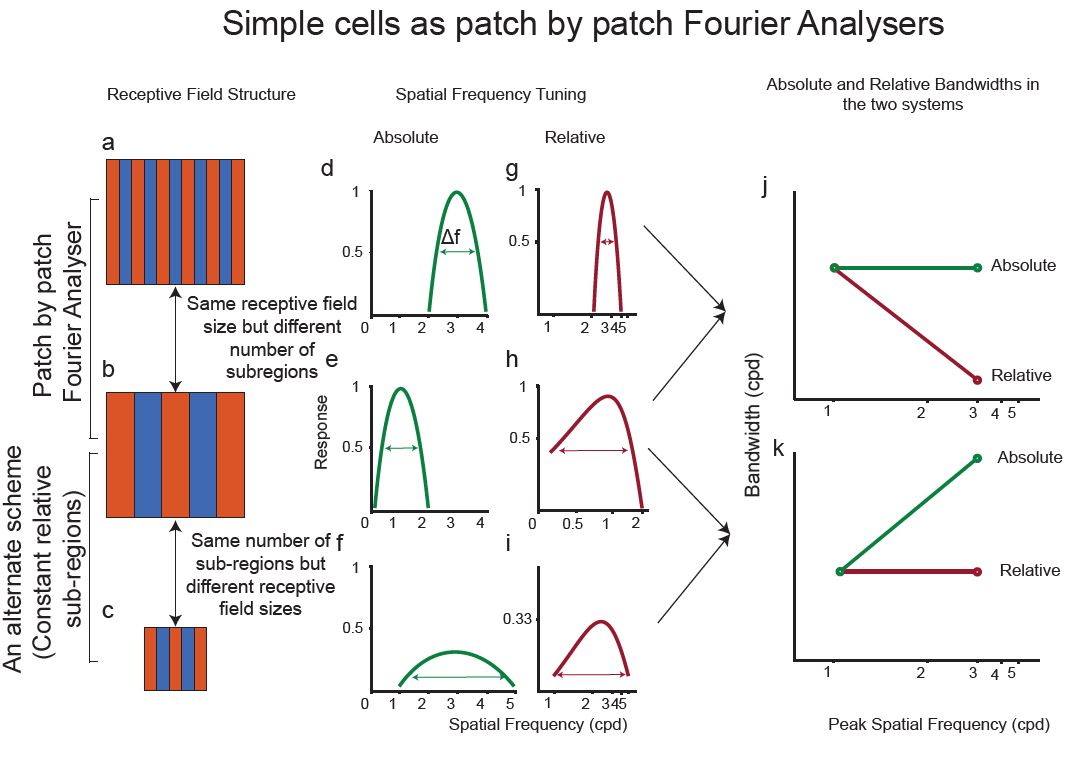
\includegraphics[width=\linewidth]{LinearV1/scheme.jpg}
		\caption{An explanation of the patch- by-patch fourier analysis model and comparison with an alternate model where the number of receptive field subregions
			and not the size of the receptive field are kept constant. (a-c) show the two-dimensional profiles of the receptive fields. (d-f) show the spatial		frequency tuning of the cells on a linear scale. The tuning bandwidth thus obtained is the absolute bandwidth. (g-i) shows the same data in (d-f)
			on a logarithmic scale. The bandwidth thus obtained is similar to the relative bandwdth. The top two rows indicate a patch by patch fourier analysis
			system. The relationship of the absolute and relative bandwidths of the neurons in this system are shown in j). The bottom two rows suggest an alternate
			scheme where the neurons have a constant number of sub-regions. The relationship between the absolute and relative bandwidths of the cells in
			this system are shown in (k).}
		\label{fig:summary}
	\end{figure}

	Despite these proposed refinements and drawbacks of the patch-by-patch spatial filter model, the idea of spatial frequency channels in visual processing has remained fairly popular. Studies have shown that the different spatial frequency channels are implicated in attentional mechanisms (References), in the perception of letters based on the size of the letters (Reference). Similarly, low spatial frequency channels have been implicated in the perception of global signals while high spatial frequency channels have been implicated in the perception of local signals. Similarly, low spatial frequency signals help identify faces while high spatial frequency signals help identify emotions. Finally, it has been suggested that spatial frequency channels are essential in analysing and perceiving natural images (Reference). In this experiment, we aim to determine if V1 simple cells in tree shrews undertake patch by patch Fourier analysis or if instead, they demonstrate constant relative subregions.
	
	While several studies have examined orientation selectivity in the tree shrew primary visual cortex, few studies have looked at spatial frequency tuning of V1 neurons. To our knowledge, only one study has reported the spatial frequency tuning of neurons in the V1 of shrew cortex. Van Hooser and colleagues showed that layer 2/3 neurons were more bandpass-tuned when compared to layer 4 neurons. Their results indicated that between 10$^o$ and 30$^o$ of eccentricity, the peak spatial frequency was between 0 and 1 cpd for most neurons and the high cut-off spatial frequency was less than 1. They also showed that where the bandwidth of neurons could be calculated, the layer 2/3 neurons had narrower bandwidths when compared to layer 4 neurons. Additionally, we here have the data to examine if the peak spatial frequencies in an orientation column remains the same indicating the presence of spatial frequency columns as has been previously suggested in cats (References) and monkeys (References).
	
	As mentioned earlier, neurons in the primary visual cortex can be classified as simple or complex cells. The criteria mentioned by Hubel and Wiesel (1962) are all subjective methods of classifying cells into simple cells. Since then, more objective methods of classifying receptive fields into simple and complex have been established. The first method is by calculating the modulation index (MI). The MI is the ratio between the DC and first harmonic component of the temporal modulation neurons exhibit when shown drifting gratings. This method quantifies the “linearity” of a neurons response based on the assumption that simple cells show linear summation within their receptive field sub-regions. Skottun et al (1991) showed that this method successfully divided neurons into two groups which were roughly the same as simple and complex cells divided using the criteria specified by Hubel and Wiesel (1962). While the modulation index measured the linearity of the neurons in cats, in macaques and tree shrews, it tended to overestimate the number of simple cells found. In tree shrews, while over 40\% of neurons could be classified as simple using the modulation index, these neurons did not show the segregation of receptive field sub-regions requisite of simple cells (Van Hooser et al., 2013; Veit et al., 2013).
	
	An alternate method of classifying neurons into simple or complex objectively is by calculating the degree of segregation of the receptive fields using the segregation index (SI). Using this method, normally, fewer units are classified as simple. Using another method of measuring receptive field subregion overlap which involved sparse noise stimuli, Viet et al (2014) only classified 9\% of neurons as simple cells. Van Hooser et al (2013) also used the SI to classify neurons into simple or complex and found a slightly larger proportion. However, they still reported that a smaller number of neurons were classified as simple using SI when compared to the MI. Our results are also compared to these previously published results.
	
	In this study, we intend to use MI and SI individually and together to determine if V1 simple cells in tree shrew perform patch by patch Fourier analysis or demonstrate constant relative sub-regions. We hypothesise that as in macaques, the tree shrews will show constant relative sub-regions.
	
	\section{Methods}
	
	\subsubsection{Surgery and Anaesthesia}
	
	As mentioned in the previous chapter, the following surgical procedures were were performed for chapters 5 and 6. Surgical procedures are as outlined in the Methods chapter. Briefly, the animal was anaesthetized using a mixture of Ketamine and Xylazine, a venous catheter was inserted in to the femoral vein and a tracheostomy performed to assist in breathing during the experiment. The animal was administered muscle paralysant (Vecuronium Bromide) intravenously and was anaesthetised using Isoflurane (0.5-1\%) for the duration of the experiment. Hard contact lenses were fitted to the eye to prevent corneal drying. In some tree shrews, additional lenses were used to correct for any refractive errors. A craniotomy and durotomy were performed over the location of V1 (Horsley-Clarke Co-ordinates A2.5 to P2.5). ECG and frontal EEG were monitored during the experiment. At the end of the experiment, the animal was euthanized using an overdose of pentobarbital sodium and perfused using 0.1M Phosphate Buffer (PB) solution followed by 4\% Paraformaldehyde in 0.1M PB. The brain was removed and stored in sucrose (20-25\%) for histology.	
	
		\subsubsection{Electrophysiology}
		High impedence, lacquer coated tungsten microelectrodes (FHC Metal Microelectrodes Inc., ME, USA; impedance= 12-18 MΩ) were lowered into the brain at an angle perpendicular to the cortical surface. The signal was amplified and filtered (x 10,000 gain, bandpass filtered between 300-3000 Hz, A-M systems) and fed into an audio speaker as well as an analog to digital converter (Cambridge Electronic Design Limited, Cambridge, UK; digitised at 22.5 kHz). Neurons were recorded from Layers 2/3 and Layer 4. Layer 4 could be identified by a characteristic ‘swish’, first for on stimuli and then for off stimuli, in the tree shrews. Where we no longer heard the swish, we concluded that we exited layer 4 and into layer 5. Neurons in layers 5 and 6 were not recorded from. Lesions (6 μA for 6s) were made at the end of each track. The electrode was withdrawn and lesions were made at regular intervals to trace the path of the electrode through the brain. The data was recorded as a spike trace using the spike 2 software (CED, Cambridge, UK). The spikes were templated and the spike timing exported as a text file. Further analysis was performed using custom MATLAB code (The Mathworks Inc, USA).
		\subsubsection{Stimuli}
		A hand-held projectoscope was used to mark the receptive field boundaries. Using this, the centre of the monitor was aligned with centre of the receptive field prior to stimulus presentation. Stimuli were presented using a BARCO monitor (Frame Refresh Rate= 80 Hz; Reference Calibrator Plus; Barco Video and Communications, Belgium) and generated using Visage (VSG, Cambridge Research Systems, Cambridge, UK) and custom Stimulus Description Language (SDL) scripts. The monitor had a mean luminance of 32.6 cdm-2. While recording, the monitor was placed at a distance of 114 cm from the eye. For each of the different stimuli described below, ten complete stimulus presentations were completed.
				\paragraph{Bar Stimuli}
				For each neurons, an initial estimate of optimum orientation was obtained using bars, moving bi-directionally across the screen. The background was a uniform gray screen. Depending on the polarity of the neurons, either a bright bar or a dark bar was used (contrast= 100 \%). The bar was usually 8o long (ranging between 4 and 8 degrees) and 0.5o wide (ranging between 0.1 and 1 degree). A total of 18 different orientations were tested and PSTHs (see methods) were made online using the Spike 2 software. The orientation that yielded the highest firing rate was used for further testing.
				After determining optimum orientation, bidirectional, dark and light (decreasing and increasing contrast) bars of the optimum orientation were used to get the response profile of the neurons to opposite polarities (see Fig. 1). 
				\paragraph{Grating Stimuli}
				For all neurons, once optimum orientation was determined, spatial frequency tuning of the neurons were studied. Drifting sine-wave gratings (TF= 4Hz, Contrast=100\%) of increasing spatial frequencies (between 0 and 2.2 cpd) and in the optimum orientation were presented to neurons. The responses were recorded and stored for further analysis.
				
   		\subsubsection{Data Analysis}
		Regardless of the stimulus presented, the following analysis was performed on the extracellular trace before any specific analysis was undertaken. Spikes were templated and the spike time and stimulus markers were exported into text files. Using custom scripts in MATLAB, PSTHs (bin-width= 20ms) were constructed for each of the stimulus conditions.  Spike density functions were created using a moving Gaussian envelope with σ of 60 ms (3 bins). This SDF was used for further analysis. 
				\paragraph{Analysis of Bar Stimuli Responses}
				Orientation tuning was analysed and presented in an earlier chapter. Here is the method by which the dark and light bar data was analysed.
					\subparagraph{Calculating Segregation Index (SI)}
					For neurons where dark and light bar data was available, the segregation index (SI) was calculated using the following formula: 
					\[SI=\frac{\sum|R_ton-R_toff|}{\sum|R_ton+R_toff|}\]
					Where, R\_ton is the response of the neuron to a light bar and R\_toff is the response of the neuron to a dark bar (see figure 1). The resulting value was a number between 0 and 1. Neurons with high segregation index (>0.5) were more likely to have segregated dark and light sub-regions and were hence categorised as simple cells. Likewise, neurons with low segregation indices were classified as complex cells as they were less likely to have segregated dark and light sub-regions.
					
					For the neurons where dark and light bar responses were present, the bimodality index was also calculated. The bimodality index was calculated for each direction of motion of the bar and the average of the two directions was taken. The BI for each direction was calculated as follows.
					
					\[BI=\frac{maxON-maxOFF}{maxON+maxOFF}\]
					
					where maxON was the maximum firing rate of the neuron to light bars and maxOFF was the maximum firing rate of the neuron to dark bars for each direction. Using this measure, where a neuron had a more dominant on sub-region, the BI was more positive and a more dominant off sub-region was represented by a negative number. The closer the number was to zero, the more likely the neuron showed equal responses to light and dark bars.
				
				\paragraph{Analysis if Grating Stimuli Responses}
				
				For all neurons, a discrete fourier transform was applied to the PSTH using the MATLAB fast fourier transform algorithm (FFT). The DC (F0) and the first harmonic component (F1) of the response was used for further analysis. Optimum spatial frequency for the neurons was determined as explained in Chapter 4. The modulation ratio was then calculated as follows.
				
				\[Modulation Index (MI)= 2*\frac{F_1}{(F_1+F_0)}\]
				
				Where Rf1 and Rf0 are the responses of the F0 and F1 components at the peak spatial frequency.
				The modulation ratio returned a number between 0 and 2. If the neuron had a modulation index greater than 1, it was classified as simple and it was classified as complex otherwise (Van Hooser et al., 2013). Only neurons classified as simple cells were used for further analysis and only the F1 component of the responses were further analysed.
				
				\paragraph{Bandwidth of Spatial Frequency Tuning}
				In the previous chapter, the distribution of peak spatial frequencies was presented. Here the spatial frequency bandwidth is discussed. For each neuron, three different measures of spatial frequency tuning bandwidths were calculated. First the upper and lower cut off spatial frequencies were calculated as follows. upper cut off was calculated as the spatial frequency greater than the peak spatial frequency where the response first reaches half the maximum response. The lower cutoff was calculated similarly for spatial frequencies lower than peak spatial frequency where response first reached half the maximum response. If the response never reached half the maximum response, the neuron was classified as low pass or high pass tuned. The first was the bandwidth of spatial frequency tuning in octaves (boct). It was calculated using the following formula.
				
				\[B_{oct}=log_2\frac{f_u}{f_l}\]
				
				where, f$_u$ and f$_l$ are the upper and lower cut-off spatial frequencies.
				
				The second was the absolute bandwidth which was calculated as follows:
				
				\[B_{abs}=f_u-f_l\]
				
				Finally, the relative bandwidth was calculated using the following formula:
				
				\[B_{rel}=\frac{B_{abs}}{f_{peak}}\]
				
				where f$_{peak}$ is the optimum spatial frequency of the neurons
								
		\subsubsection{Histology}
				The brains were stained for Nissl substances using cresyl violet acetate and lesions were located. The number of neurons found in each layer have been presented in V1 chapter and are not presented here. However, for all the results presented here, layer specific results are also presented.
							
					

	\section{Results}
	
		Results from a total of 64 neurons are presented below. Where possible, the layerwise distribution is also presented. 
	

		
	\paragraph {Segregation Index}	
	In 49 of the 64 neurons, we recorded the response of the neuron to dark and light bars. Simple cells have segregated receptive fields which appear as separate peaks in the PSTHs (Fig 1a) and complex cells have overlapping subregions which appear as overlapping peaks in the PSTH (Fig 1b). Accordingly, the segregation index is higher for simple cells compared to complex cells.
	
		\begin{figure}[]
		
		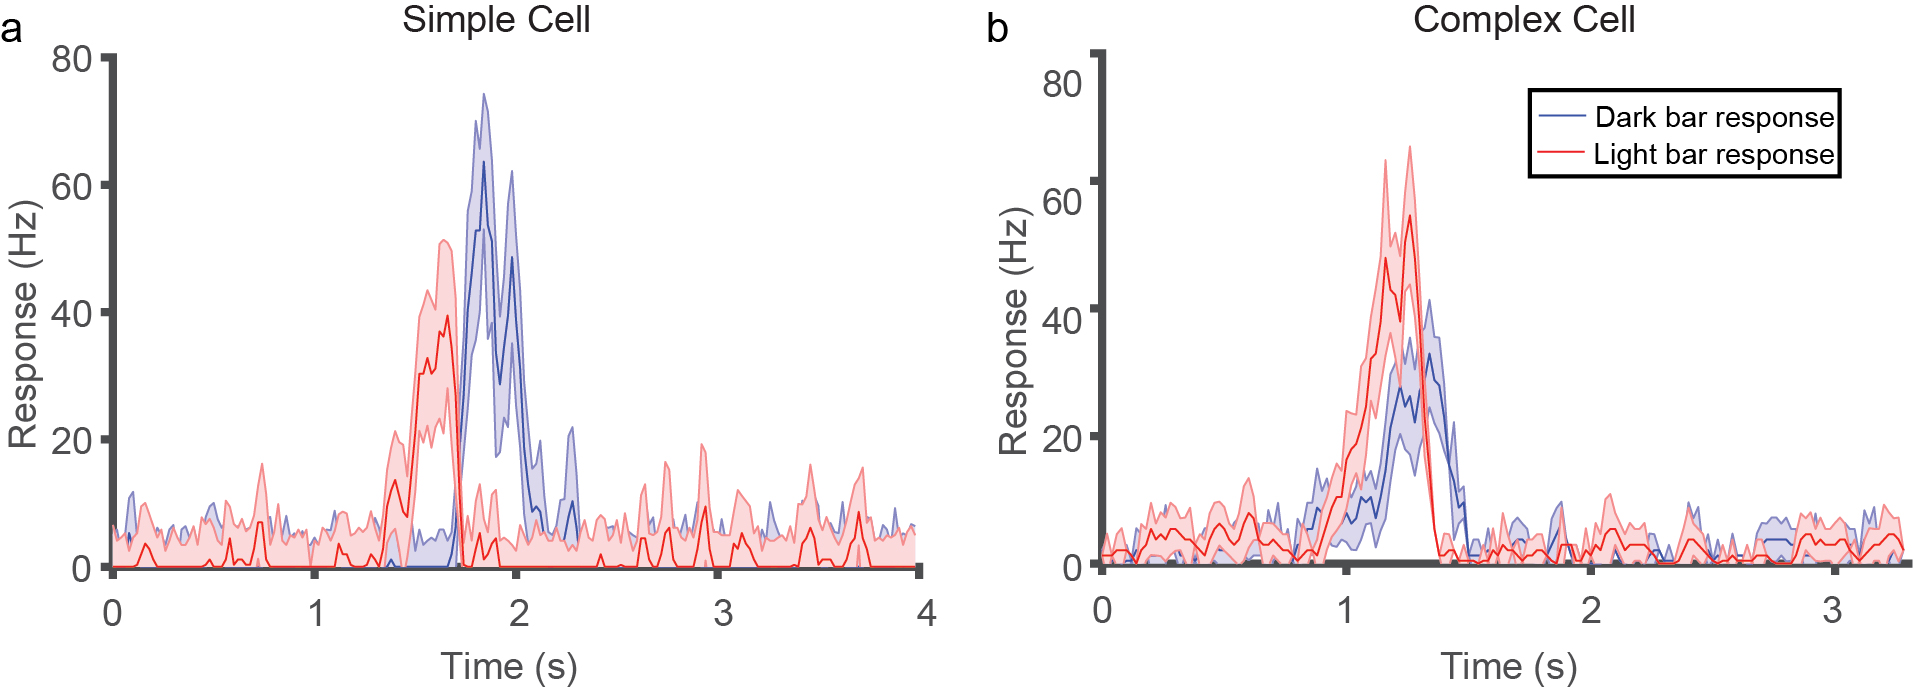
\includegraphics[width=\linewidth]{LinearV1/simplecomplex.jpg}
		\caption{Response of a simple (a) and complex cell (b) to the dark and light bar stimuli. The spatially segregated RF of the simple cells is translated into the temporally segregated response of the neuron. Whereas, in the complex cell, the overlapping sub-regions are reflected in the temporally overlapping response of the neuron. Accordingly, the simple cell has a high SI (0.92) and the complex cell has a lower SI (0.39).}
		\label{fig:fig2}
	\end{figure}
	
	The distribution of segregation index for 47 neurons is presented below. Of the 49 neurons, 19 were from layer 2/3, 12 were from layer 3c and 18 were from layer 4. There was no significant difference in SI between the layers (Kruskal-Wallis test, p=0.34).

	\begin{figure}[]
		
		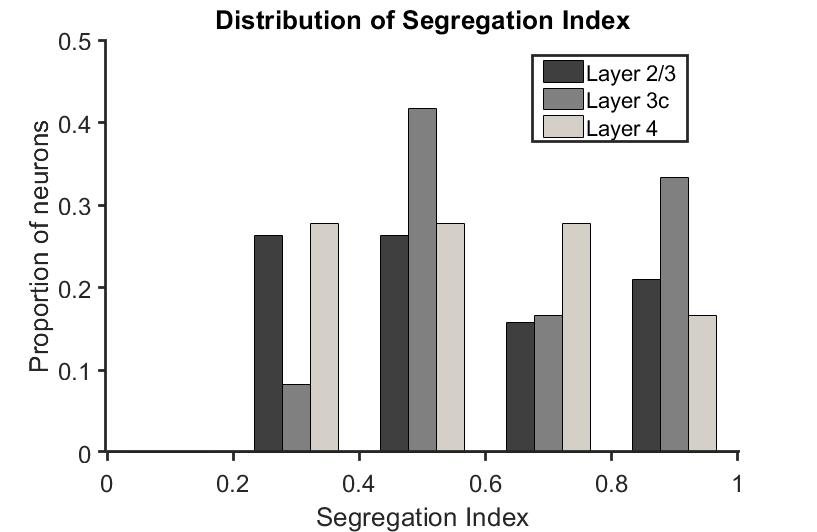
\includegraphics[width=\linewidth]{LinearV1/segregationindex_colouradj.jpg}
		\caption{Distribution of segregation indices of neurons.}
		\label{fig:fig3}
	\end{figure}

	\paragraph{Bimodality Index}
	
	The distribution of the bimodality index for the neurons in each of the layers are shown below. As with the segregation index, there was no significant difference in the distribution of the bimodality index between the three layers (Kruskal-Wallis test, p=0.49).
	
	\begin{figure}[]
		
		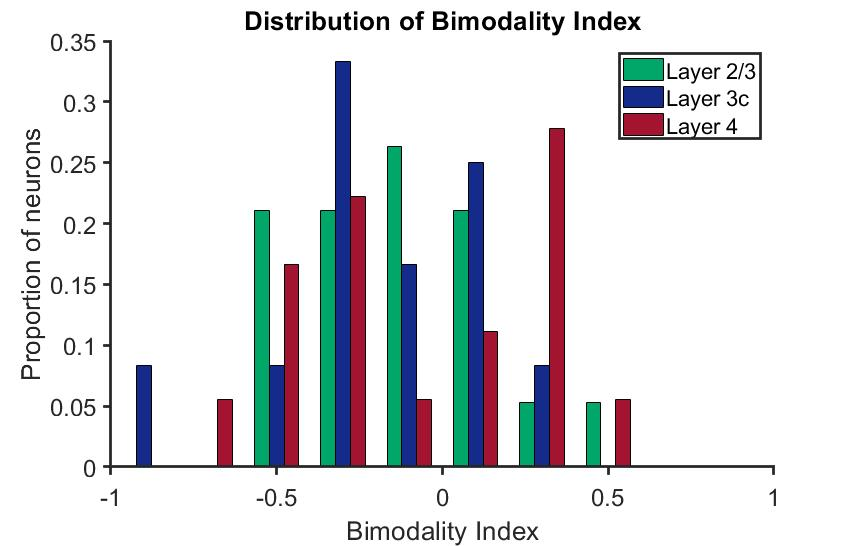
\includegraphics[width=\linewidth]{LinearV1/Biindex.jpg}
		\caption{Distribution of bimodality indices of neurons.}
		\label{fig:bi}
	\end{figure}

	\paragraph{Modulation Index}
	The modulation indices of all the 69 neurons [Layer 2/3= 27; Layer 4= 27; Layer 3c= 15] are shown in figure 3. There was no significant difference in the modulation index between the layers (Kruskal-Wallis test, p= 0.74).
	
		\begin{figure}[]
		
		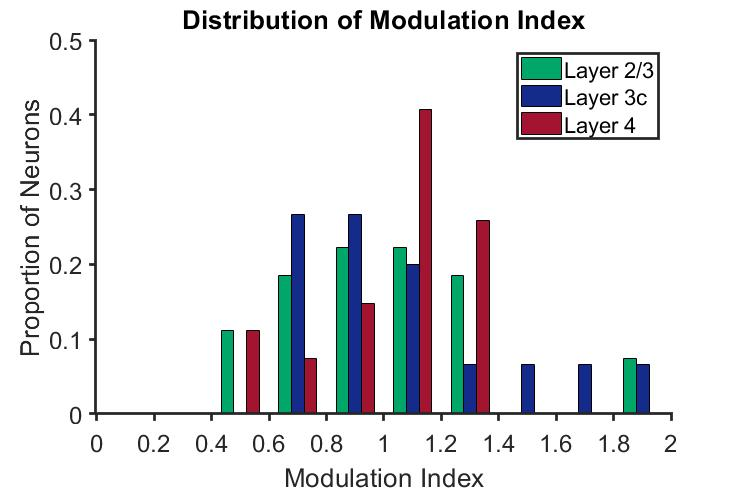
\includegraphics[width=\linewidth]{LinearV1/modind_layer_colour.jpg}
		\caption{Distribution of modulation indices of neurons.}
		\label{fig:fig4}
	\end{figure}


	In neurons where both the segregation index and modulation index were recorded, they were plotted against each other. There was no significant correlation between the two indices (rho=0.02, p=0.89). 
	
	
	\begin{figure}[]
		
		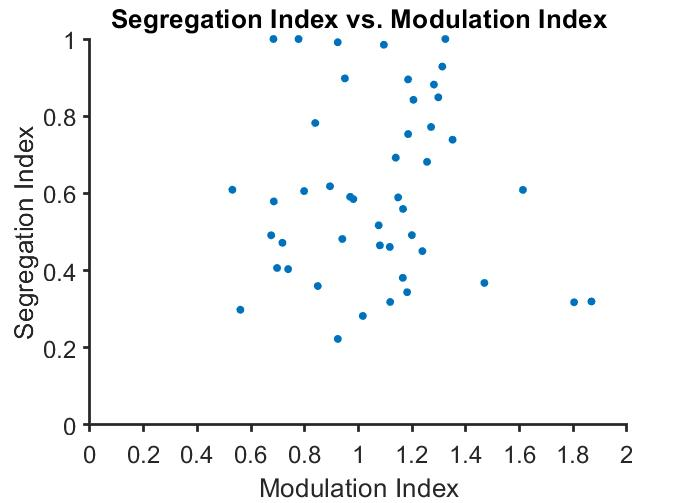
\includegraphics[width=\linewidth]{LinearV1/Segindvsmodind.jpg}
		\caption{Relationship between the modulation and segregation indices. The horizontal line is the threshold for the SI, where neurons above the threshold are classified as simple. The vertical line is the threshold between the simple and complex cells using the Modulation Index. If the segregation index and modulation index both classified the same neurons as simple and complex, we will only expect neurons to fall into the bottom left and the top right quadrants, unlike the distribution seen here.}
		\label{fig:fig5}
	\end{figure}

	It might be useful to discuss neurons in the two quadrants where one method classifies them as simple while the other doesn't. In the top left quadrant, when using the segregation index, the neurons will be classified as simple but when using the MI, the neurons will be labelled complex (A total of 11 neurons). Most of these neurons were in layers 4 and layer 3c but apart from this, there were no clear patterns visible in the data.
	
	The neurons in the bottom right corner will be classified as simple using the modulation index but not using the segregation index (11 neurons). The majority of these neurons were from layer 4(7/11) and most neurons had a negative bimodality index, indicating that they were off dominated neurons (8/11). These neurons also tended to have receptive fields dominated by one polarity as shown in fig\ref{fig:conc}.
	
		\begin{figure}[]
		
		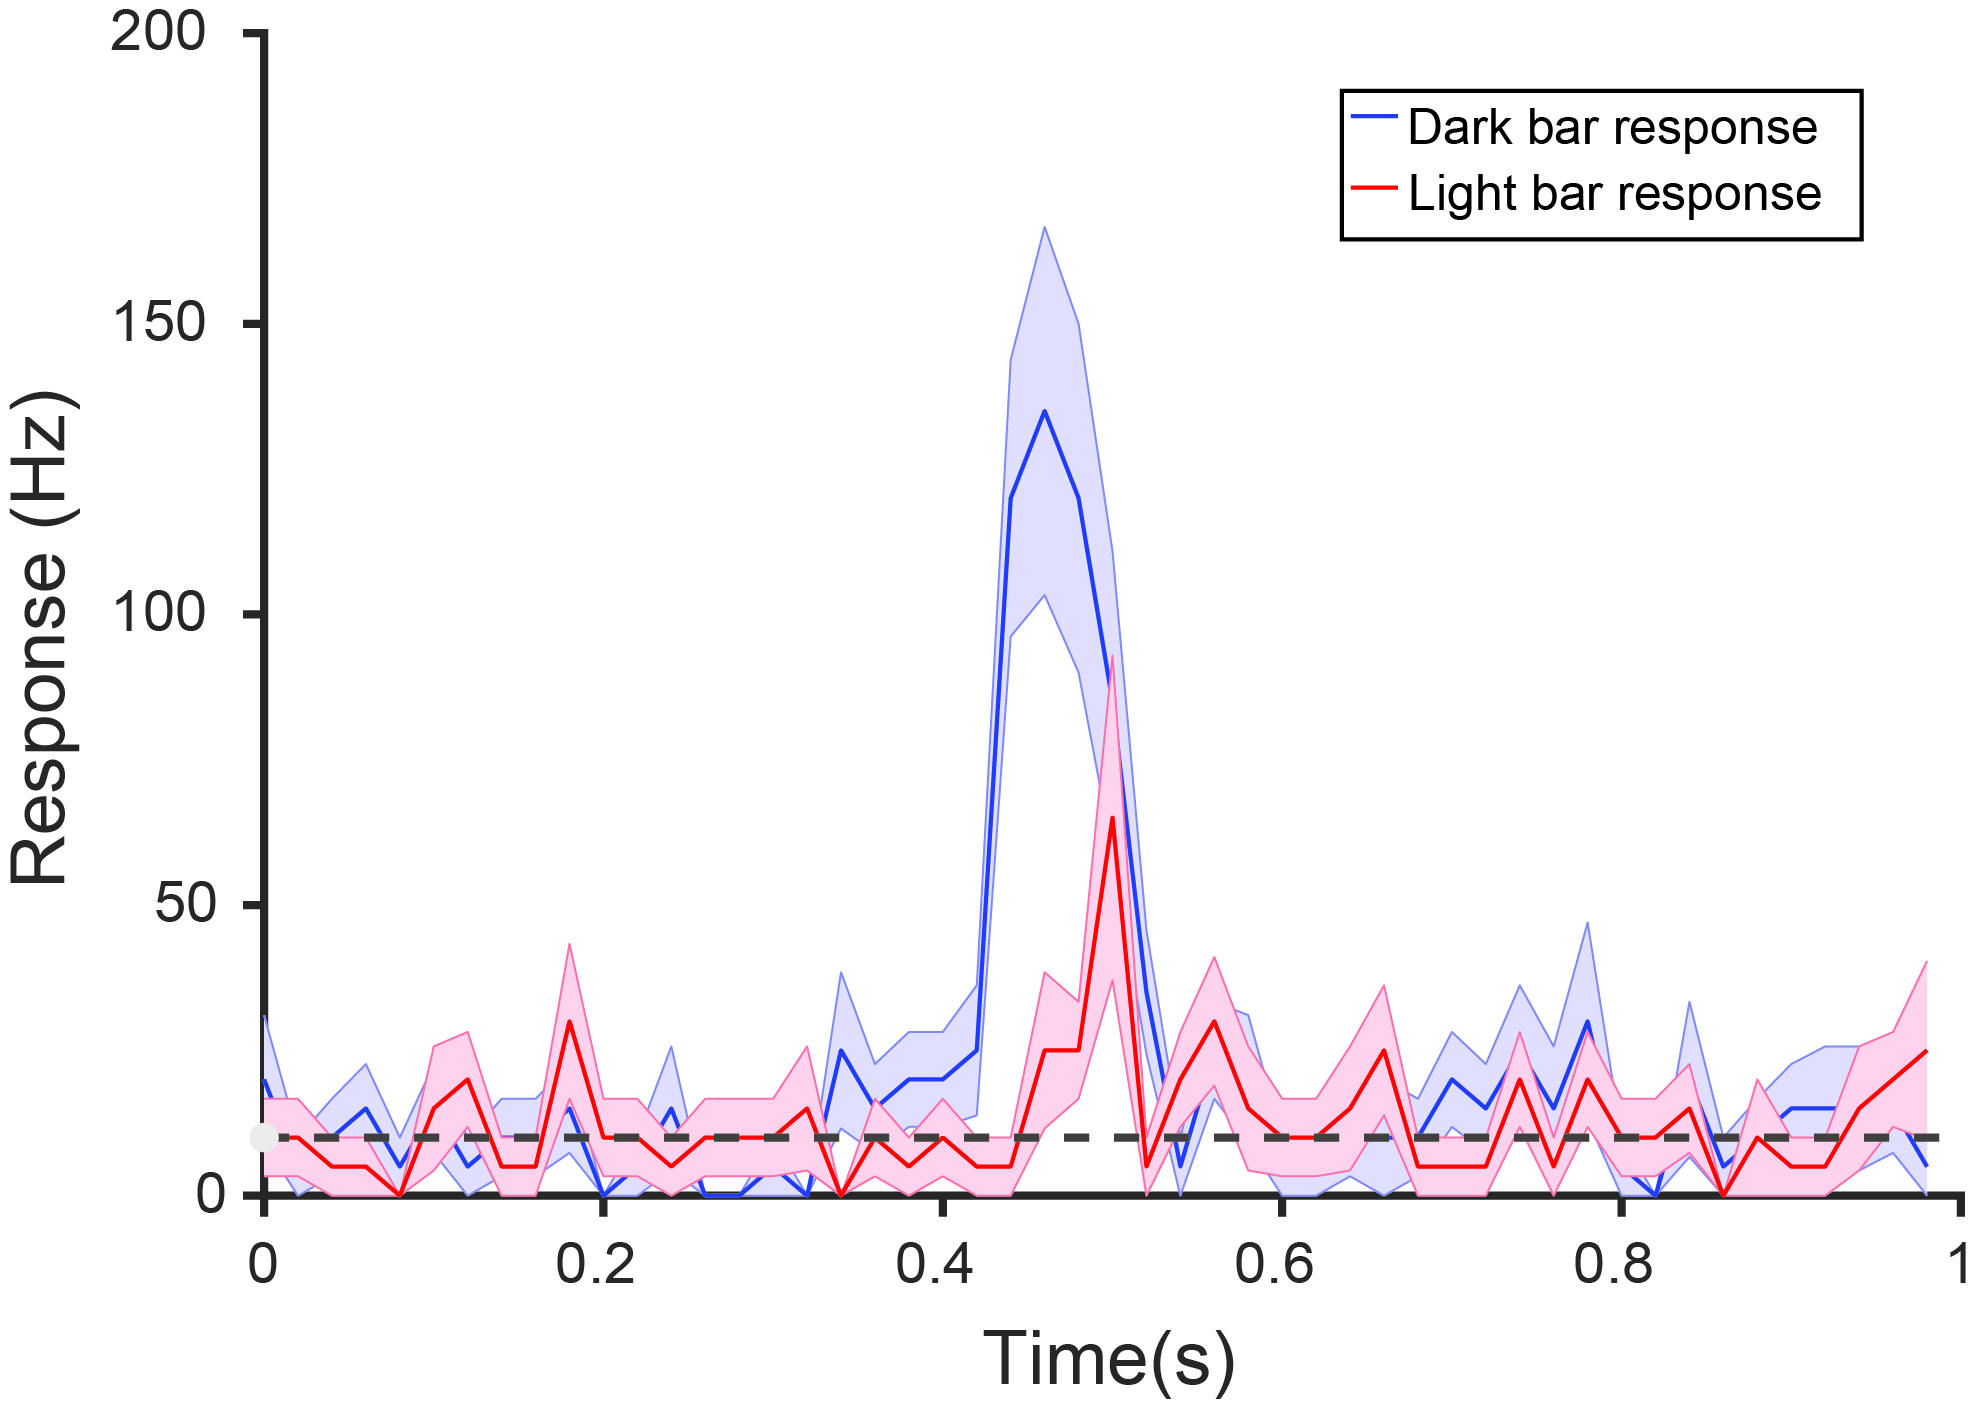
\includegraphics[width=\linewidth]{LinearV1/concneurons.jpg}
		\caption{A neuron that responds preferably to a dark bar. This neuron has a segregation index less than 0.5 but still shows modulated responses to stimuli, potentially due to the imbalance in the two sub-regions. The dashed line shows the spontaneous activity of the neuron.}
		\label{fig:conc}
	\end{figure}

	\paragraph{Distribution of bandwidth in octaves}
	
	In most species studied so far, the bandwidth of SF tuning in octaves has been constant (~1.5 octave) with a large range of tuning widths. Therefore, the distribution of the bandwidth of the neurons in octaves is presented in figure \ref{fig:boct}. The data is also presented individually for neurons determined as simple and complex using the Modulation Index and the segregation Index separately (figure \ref{fig:boct}a and b).

		\begin{figure}[H]
		
		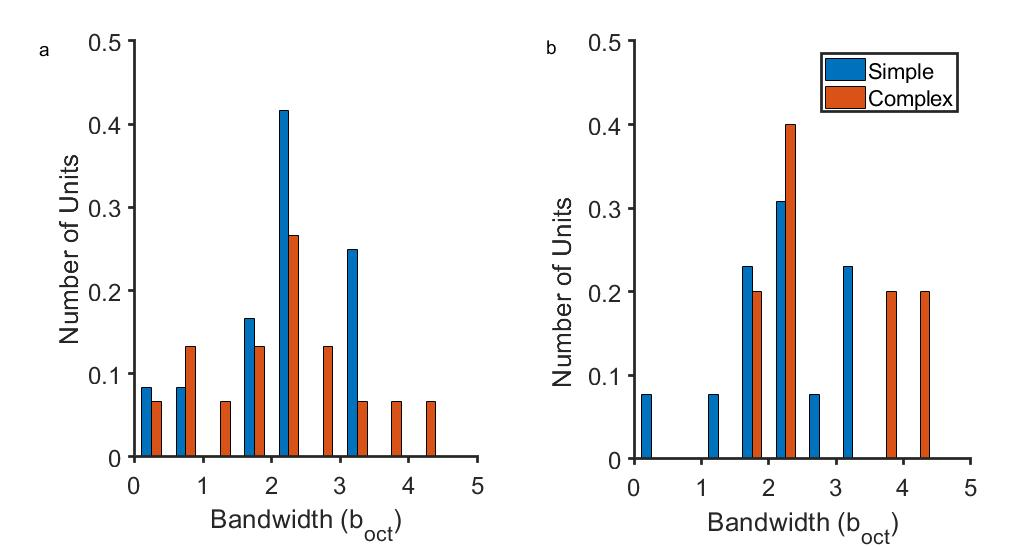
\includegraphics[width=\linewidth]{LinearV1/boct.jpg}
		\caption{The distribution of B$_{oct}$ in simple and complex cells classified using the modulation index (a) and the segregation index (b). a) }
		\label{fig:boct}
		
		\end{figure}
	
	The median b$_{oct}$ for both simple and complex cells was 2.3 octaves with neurons responding between 0 and 4.5 octaves. 
	\paragraph{Relationship between bandwidth and spatial frequency}
	
	Neurons were classified as simple cells using the modulation index (MI$>$1), the segregation index (SI$>$0.5), both the modulation and segregation index together (MI $>$ 1 and SI $>$0.5). The relationship between the absolute bandwidth and the peak spatial frequency for simple cells classifies as described as above as well as for all the neurons in the sample are shown in figure \ref{fig:hwpksf}(a,c\&e). Statistically significant relationships are indicated using $*$. There was a significant correlation between the when all neurons were used for the analysis. The relationship between relative bandwidth and the peak spatial frequency are shown in the right hand panel. In all cases except for the one in (f) the results were statistically significant.
	
		\begin{figure}[]
		
		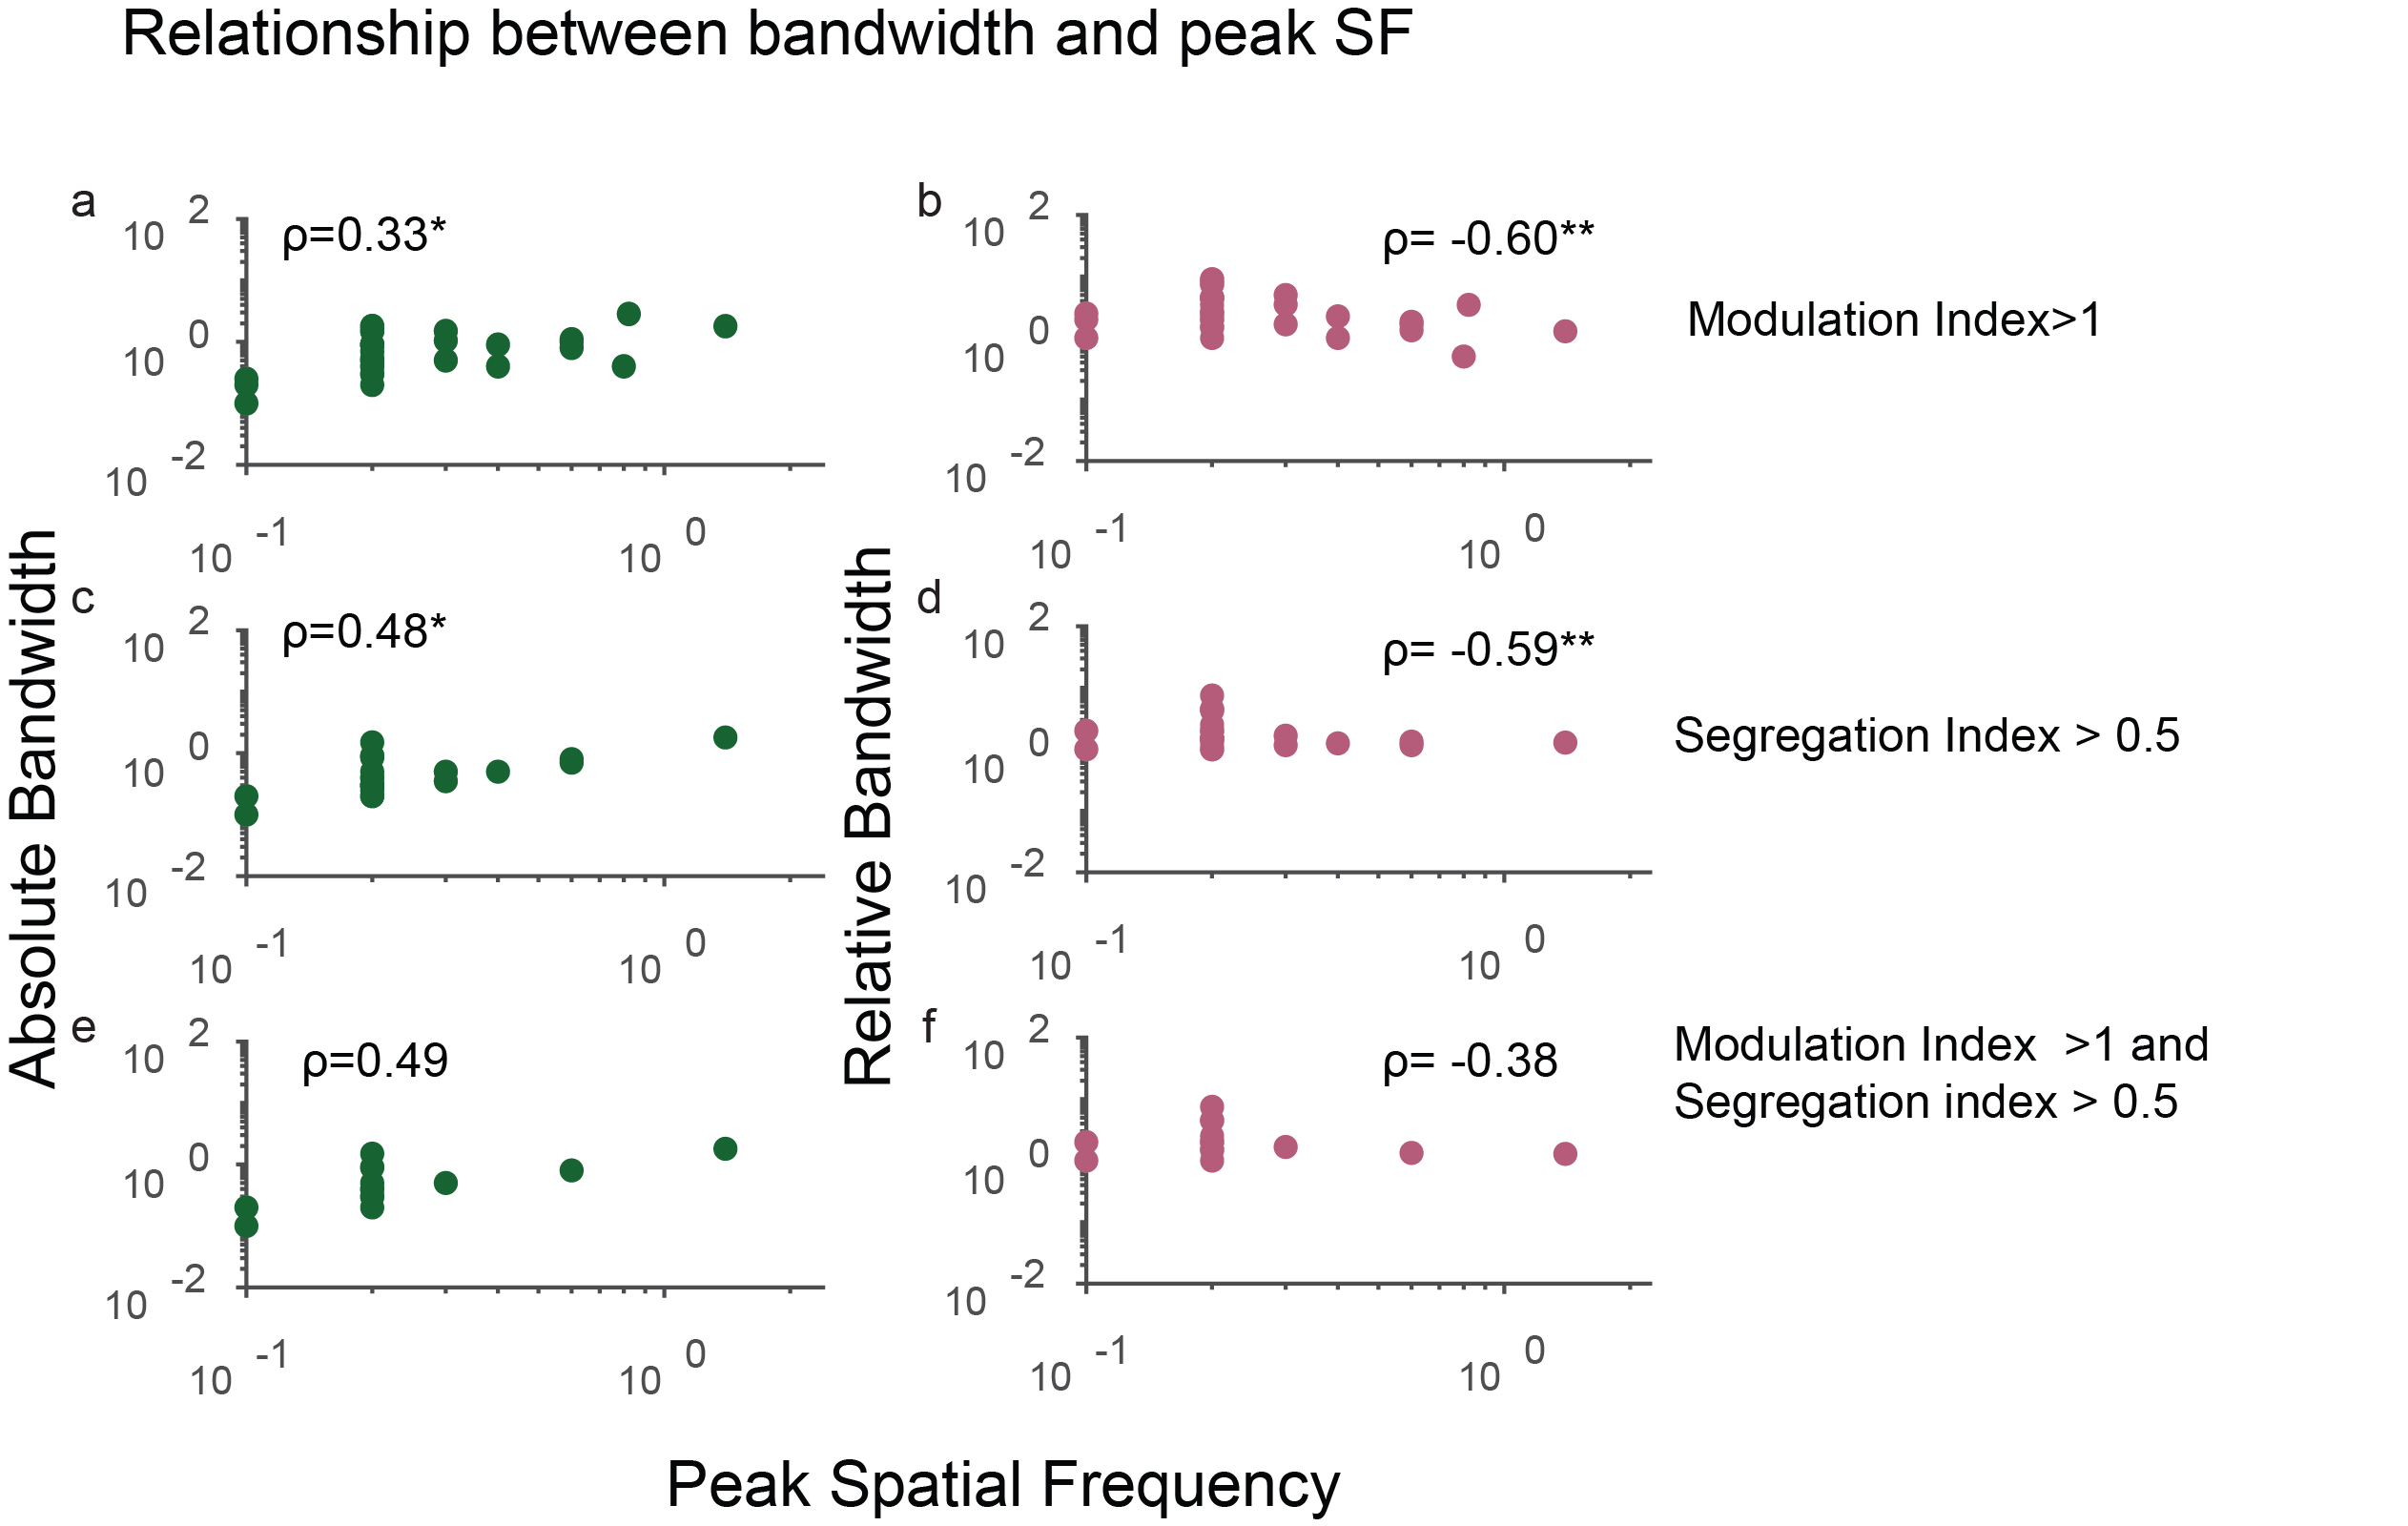
\includegraphics[width=\linewidth]{LinearV1/hwpksf2.jpg}
		\caption{This figure shows the relationship between bandwidth and spatial frequency in simple cells when using the modulation index to classify units (a,b), when using the segregation index (c,d); using both the modulation and segregation index (e,f). The plots on the left hand side show the relationship between absolute bandwidth and the peak spatial frequency while the plots on the right hand side show the relationship between the relative bandwidth and peak spatial frequency. Number of units used for generating each plot is specified in the right hand corner and statistically significant results are shown by *. *= p$<$0.05. **=p$<$0.005.}
		\label{fig:hwpksf}
		\end{figure}
	
	Further, the datapoints in the right handside plots in fig \ref{fig:hwpksf} were fit with curves and the slopes of the curves are presented below. When just the modulation index was used to classify neurons into simple cells, the slope was -0.57, when the segregation index was used, the slope was -0.76 and when both measures were used, the slope was -0.53, indicating that there is a strong negative relation between the relative bandwidth and the peak spatial frequency of the neurons.
	
	\section{Discussion}
	
	In this chapter, we investigated if V1 simple cells in the tree shrew behaved like patch by patch Fourier analysers. Our results showed that as the peak spatial frequency increased, the relative bandwidth decreased as is expected of neurons that are Fourier Analysers. This result was found regardless of the method used to classify neurons into simple and complex cells. We also found that both simple and complex cells in V1 were tuned to a bandwidth of 2.3 octaves. These results are interpreted in the context of space and spatial frequency analysis performed by the visual system below.
	
	Our first major result shows that regardless of the method of classification, simple cells in the tree shrew V1 showed a decrease in the relative bandwidth as the peak spatial frequencies increased. This is indicative of shrew V1 neurons functioning as patch by patch Fourier analysers (figure \ref{fig:summary}j). In similar analysis conducted by Kulikowski and colleagues in cats and macaques, neurons classified as silent periodic neurons were omitted from the analysis as these neurons would have been classified as linear using the modulation index despite showing strong non-linearities. Using both the SI and MI would have ensured that these neurons were omitted in the analysis. This measure also showed that the neurons in V1 acted as linear filters.
	
	However, the slope measurements suggest that these neurons are not ideal Fourier analysers. An ideal Fourier analyser would have a slope of -1 whereas using the different methods, the largest slope we could achieve was -0.76 (using Segregation Index). It has been suggested that for simple cells to be ideal Fourier analysers, they need to have infinitely narrow spatial frequency bandwidths. However, this is not always the case for the tree shrew simple cells. There are neurons that are tuned to bandwidths greater than 4 octaves in our sample. A further requirement for simple cells to be linear filters is that the different spatial frequency channels need to be independent. However, in the primary visual cortex, due to the horizontal connections present in the supragranular layers, this is difficult to achieve. In the tree shrews particularly, extensive short and long range horizontal connections have been reported in the primary visual cortex. As a result, the capacity of simple cells in any visually system may have some key physiological constraints.
	
	Kulikowski et al (1982) suggested that for simple cells to be edge detectors, they needed to have a maximum bandwidth of 1.5 octaves. In cats and macaques, most neurons have a bandwidth between the range 1.3 and 1.5 octaves, which is consistent with the claim that these neurons might undertake some degree of spatial analysis instead of a purely spatial frequency analysis. However, most neurons in the shrew V1 has a bandwidth greater than 1.5 octaved with the majority tuned to approximately 2.3 octaves. As a result, there may be lesser proportion of neurons undertaking spatial analysis and most neurons may infact be performing a Fourier analysis of the visual space. 
	
	In order to classify the neurons into simple and complex cells, we used two objective measures that are regularly used in the literature: a) The Segregation Index and b) The Modulation Index. The SI measures the degree of separateness of the receptive field sub-regions i.e., if there are separate on and off sub-regions. Using this measure, we found that about half the neurons for which this data was available for were simple. The MI on the other hand measures the degree of linear summation over the receptive fields. Using this measure too, a similar proportion of  neurons were classified as simple cells. However, there was no significant correlation between the two measures (See fig.\ref{fig:fig5}). This indicates that different neurons are classified as simple based on the two different measures. Only half the neurons that were classifies as simple using the SI were also classified as simple using the modulation index, indicating that atleast half the neurons that show linear summation over their receptive field also had overlapping sub-regions. 
	
	The distribution of SI and MI in our results show that neither of these values differ significantly across layers. The SI seems to be distributed almost uniformly across the whole range of possible values (between 0 and 1). However, it is interesting to note that no neurons showed complete and equally overlapping subregions (SI $<$ 0.2; see fig.\ref{fig:fig3}). These results are also consistent with those published by Van Hooser et al., 2013 (see fig 3c). This could mean that most neurons in the shrew V1 receive unbalanced on and off inputs. (Check Bimodality Index). Previous studies have suggested that the tree shrew V1 has a preponderance of off dominated neurons. It has also been suggested that this off dominance could be the origin of orientation selectivity in the V1 of tree shrews. Another reason for the difference could also be the way SI is calculated. The SI is calculated from the temporal profile of the neuronal response to light and dark bars. While this gives an accurate enough measure, it may not be sensitive enough to detect small differences in sensitivities between the off and on regions. A different measure of segregation index can also be calculated using ---- (Veit et al., 2014). This method uses stationery flashing stimuli to estimate the degree of segregation of the receptive fields. Using this measure, only 7\% of cortical neurons were classified as simple when compared to the 50\% using the segregation index.
	
	While the distribution of MI was not significantly different between the layers, there are a few important trends that may be of note. First, while the layer 2/3 and layer 3/c distribution look identical, a majority of Layer 4 neurons seem to have a modulation index greater than 1 (see fig.\ref{fig:fig4}). This is consistent with reports in literature where the simple cells are present predominantly layer 4 with some complex cells also found in this layer. As reported in Van Hooser et al (2013), a significant proportion of layer 2/3 neurons (layer 2/3 + Layer 3c) neurons were complex like (MI$<$1).
	
	Our results on the simple and complex cell dichotomy are similar to those reported by Van Hooser et al., 2013. They also classified an equivalent proportion of neurons into simple and complex using both the modulation index and segregation index. The relationship between the two measures wasn't reported. There are however, few results that were different, especially in regards to neurons in layer 2/3. First, Van Hooser and colleagues reported that most layer 2/3 neurons in their sample showed stronger on responses (56\%) whereas, in our sample, a larger proportion of layer 2/3 neurons showed stronger off responses (~65\%). They also found that an equivalent percentage of neurons were classified as simple using modulation index but found that a smaller proportion of neurons were classified as simple using the segregation index. They suggest that this might be due to an imbalance in the on and off sub-regions. The neurons in our sample that would have been classified as simple using the Modulation index but not so using the segregation index are shown in the bottom right quadrant in figure \ref{fig:conc}. A majority of these neurons were however located in layer 4, where such an imbalance of input is expected due to the layered segregation of on and off neurons layer 4.
	
	
	\section{Conclusion}
	
	In this study, we examined whether simple cells in the primary visual cortex of tree shrews acted as Fourier analysers or combined spatial and spatial frequency information to analyse the visual scene. We used two measures, the modulation index and the segregation index to classify neurons into simple and complex cells. We also used both measures simultaneously to classify neurons into simple and complex cells. We found that the median spatial frequency bandwidth of the neurons (simple and complex) was 2.3 octaves, which is considerably higher than those reported in cats and macaques (between 1.3 and 1.5 octaves). We also found that regardless of the method used for classifying neurons into simple and complex, simple cells responses were closer to that of linear Fourier analysers in the tree shrew. Although simple cells in the shrew V1 are not ideal Fourier analysers, they are far better when compared to cats and monkeys.